\documentclass[../main.tex]{subfiles}

\begin{document}
\section*{L4N1 Part 1}\addcontentsline{toc}{section}{L4N1 Part 1} 
\subsubsection*{ICMP}
%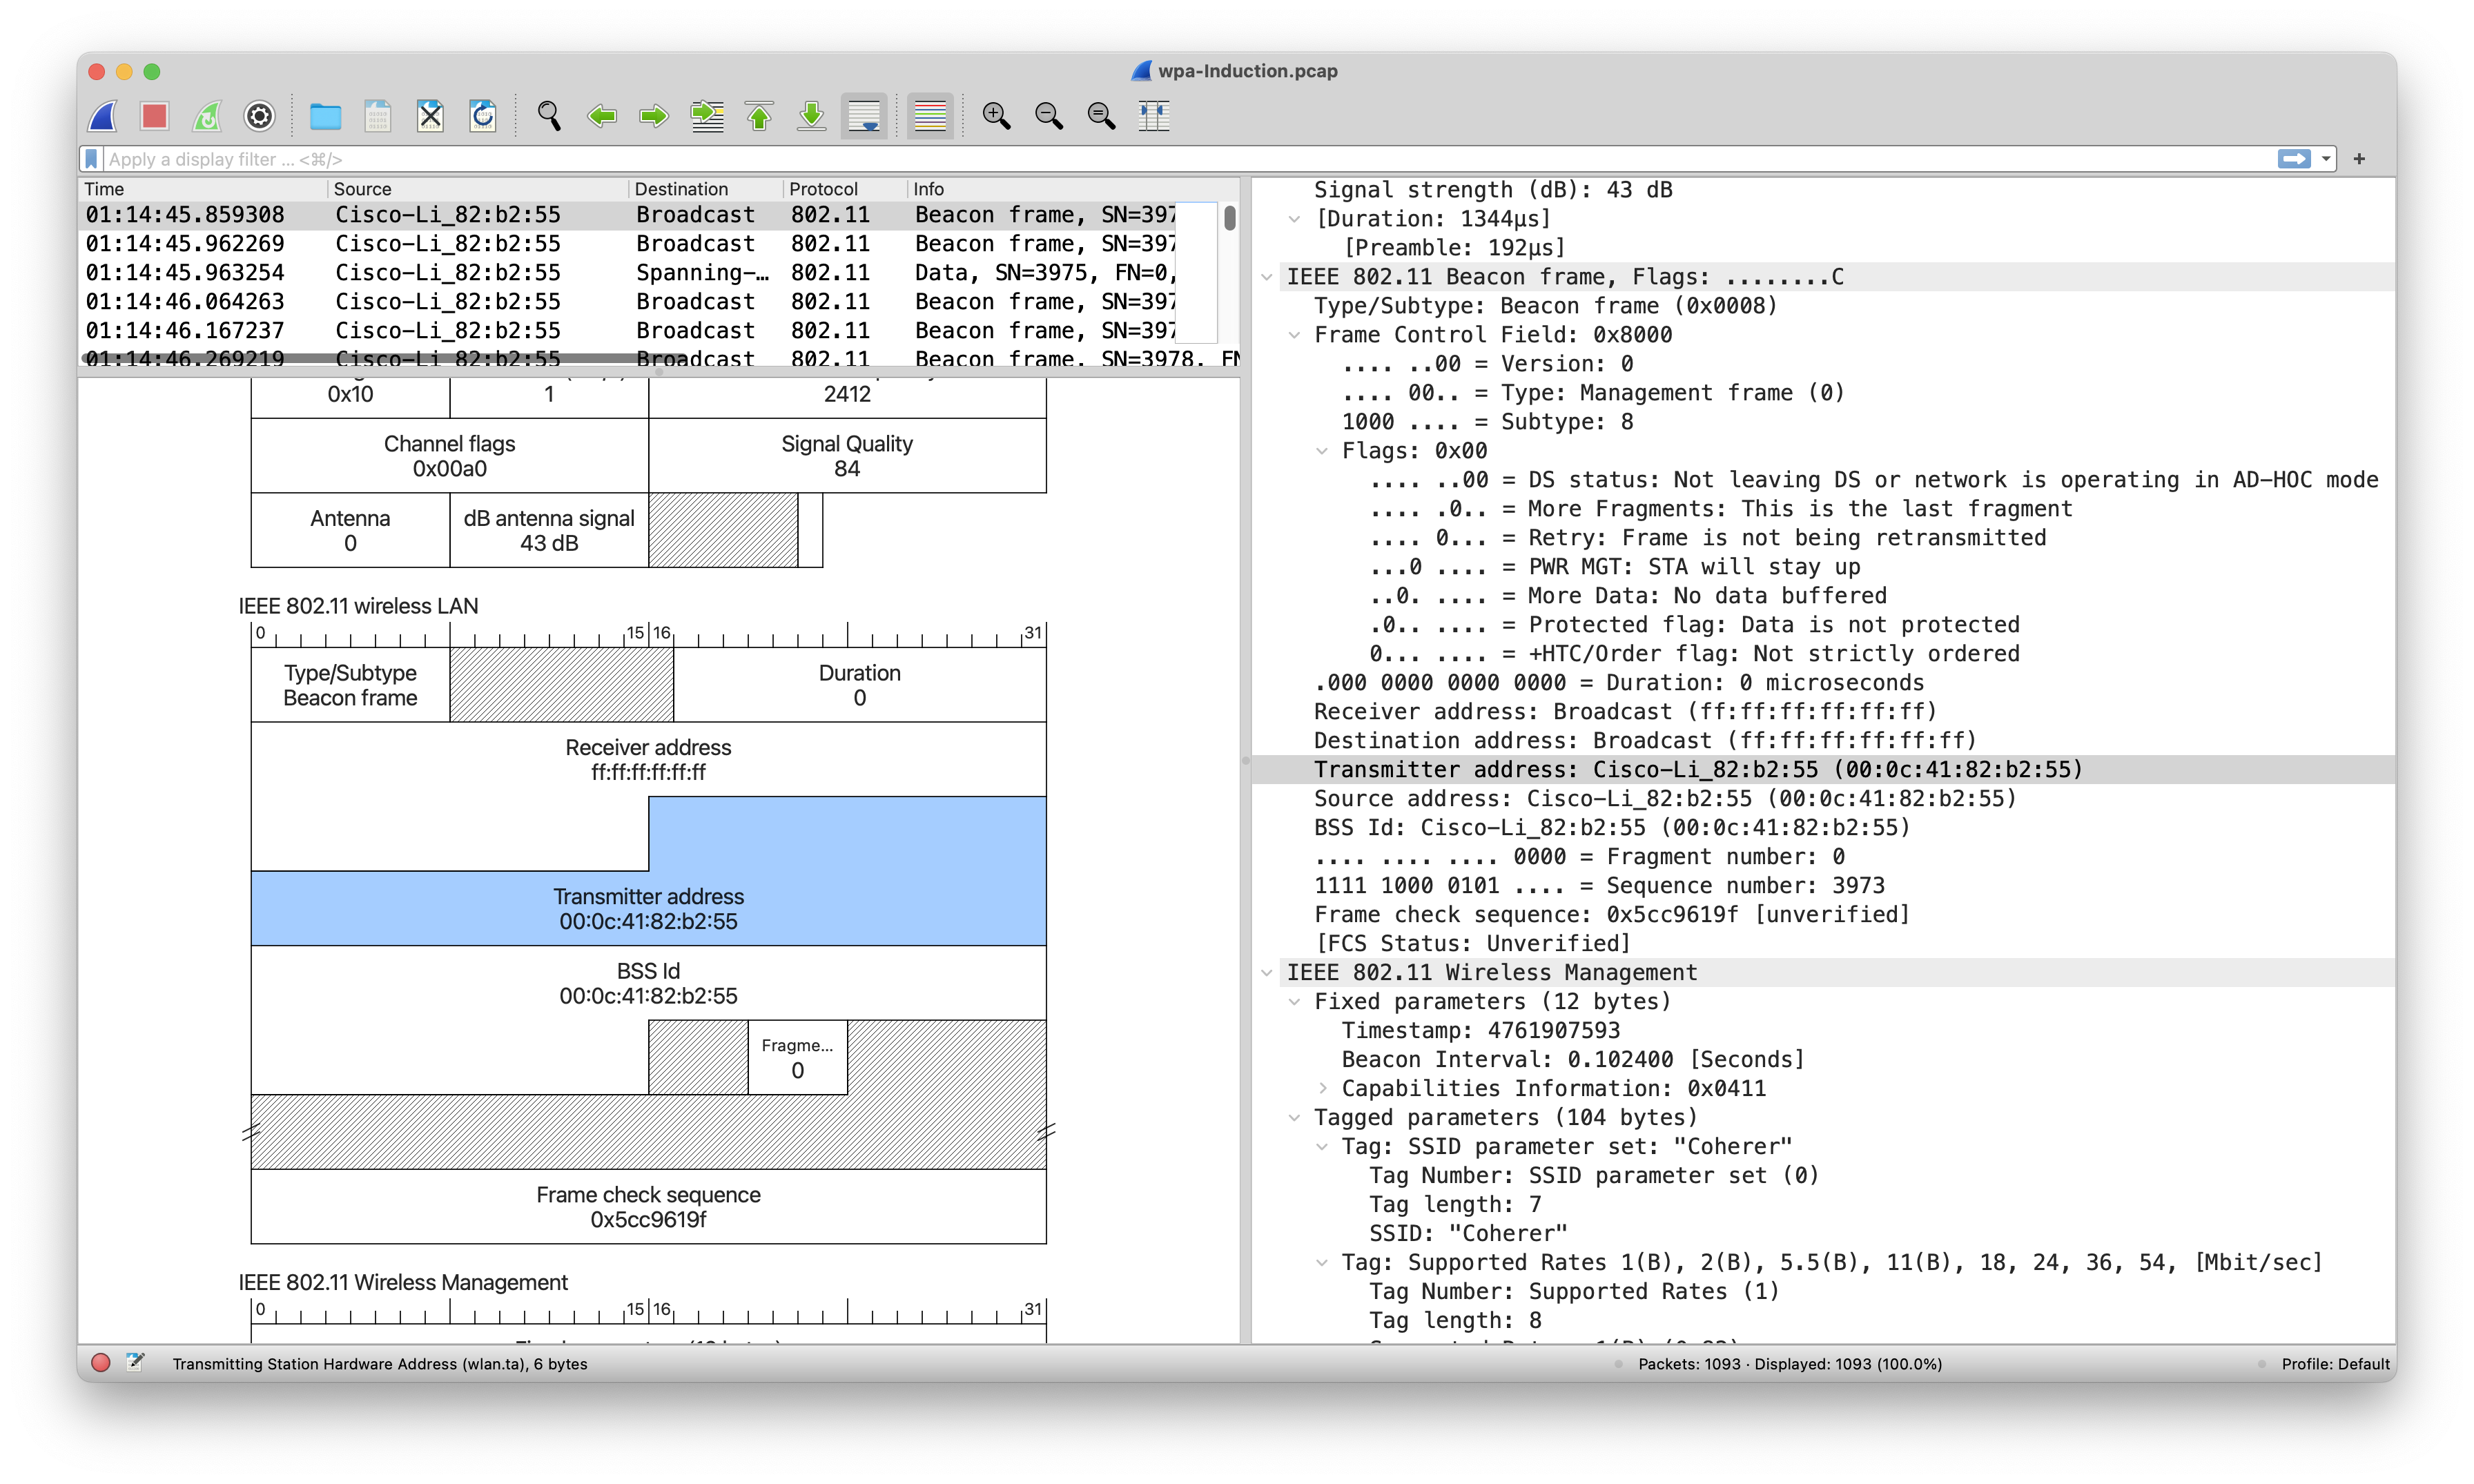
\includegraphics[width=\textwidth]{subfiles/images/PART2_Beacon_Frame.png}
\newpage
\problem{1}
\begin{wts}
    How many ICMP packets are in the list plane?
\end{wts}
\begin{proof}
    Consider the subsequent graphic.\\
    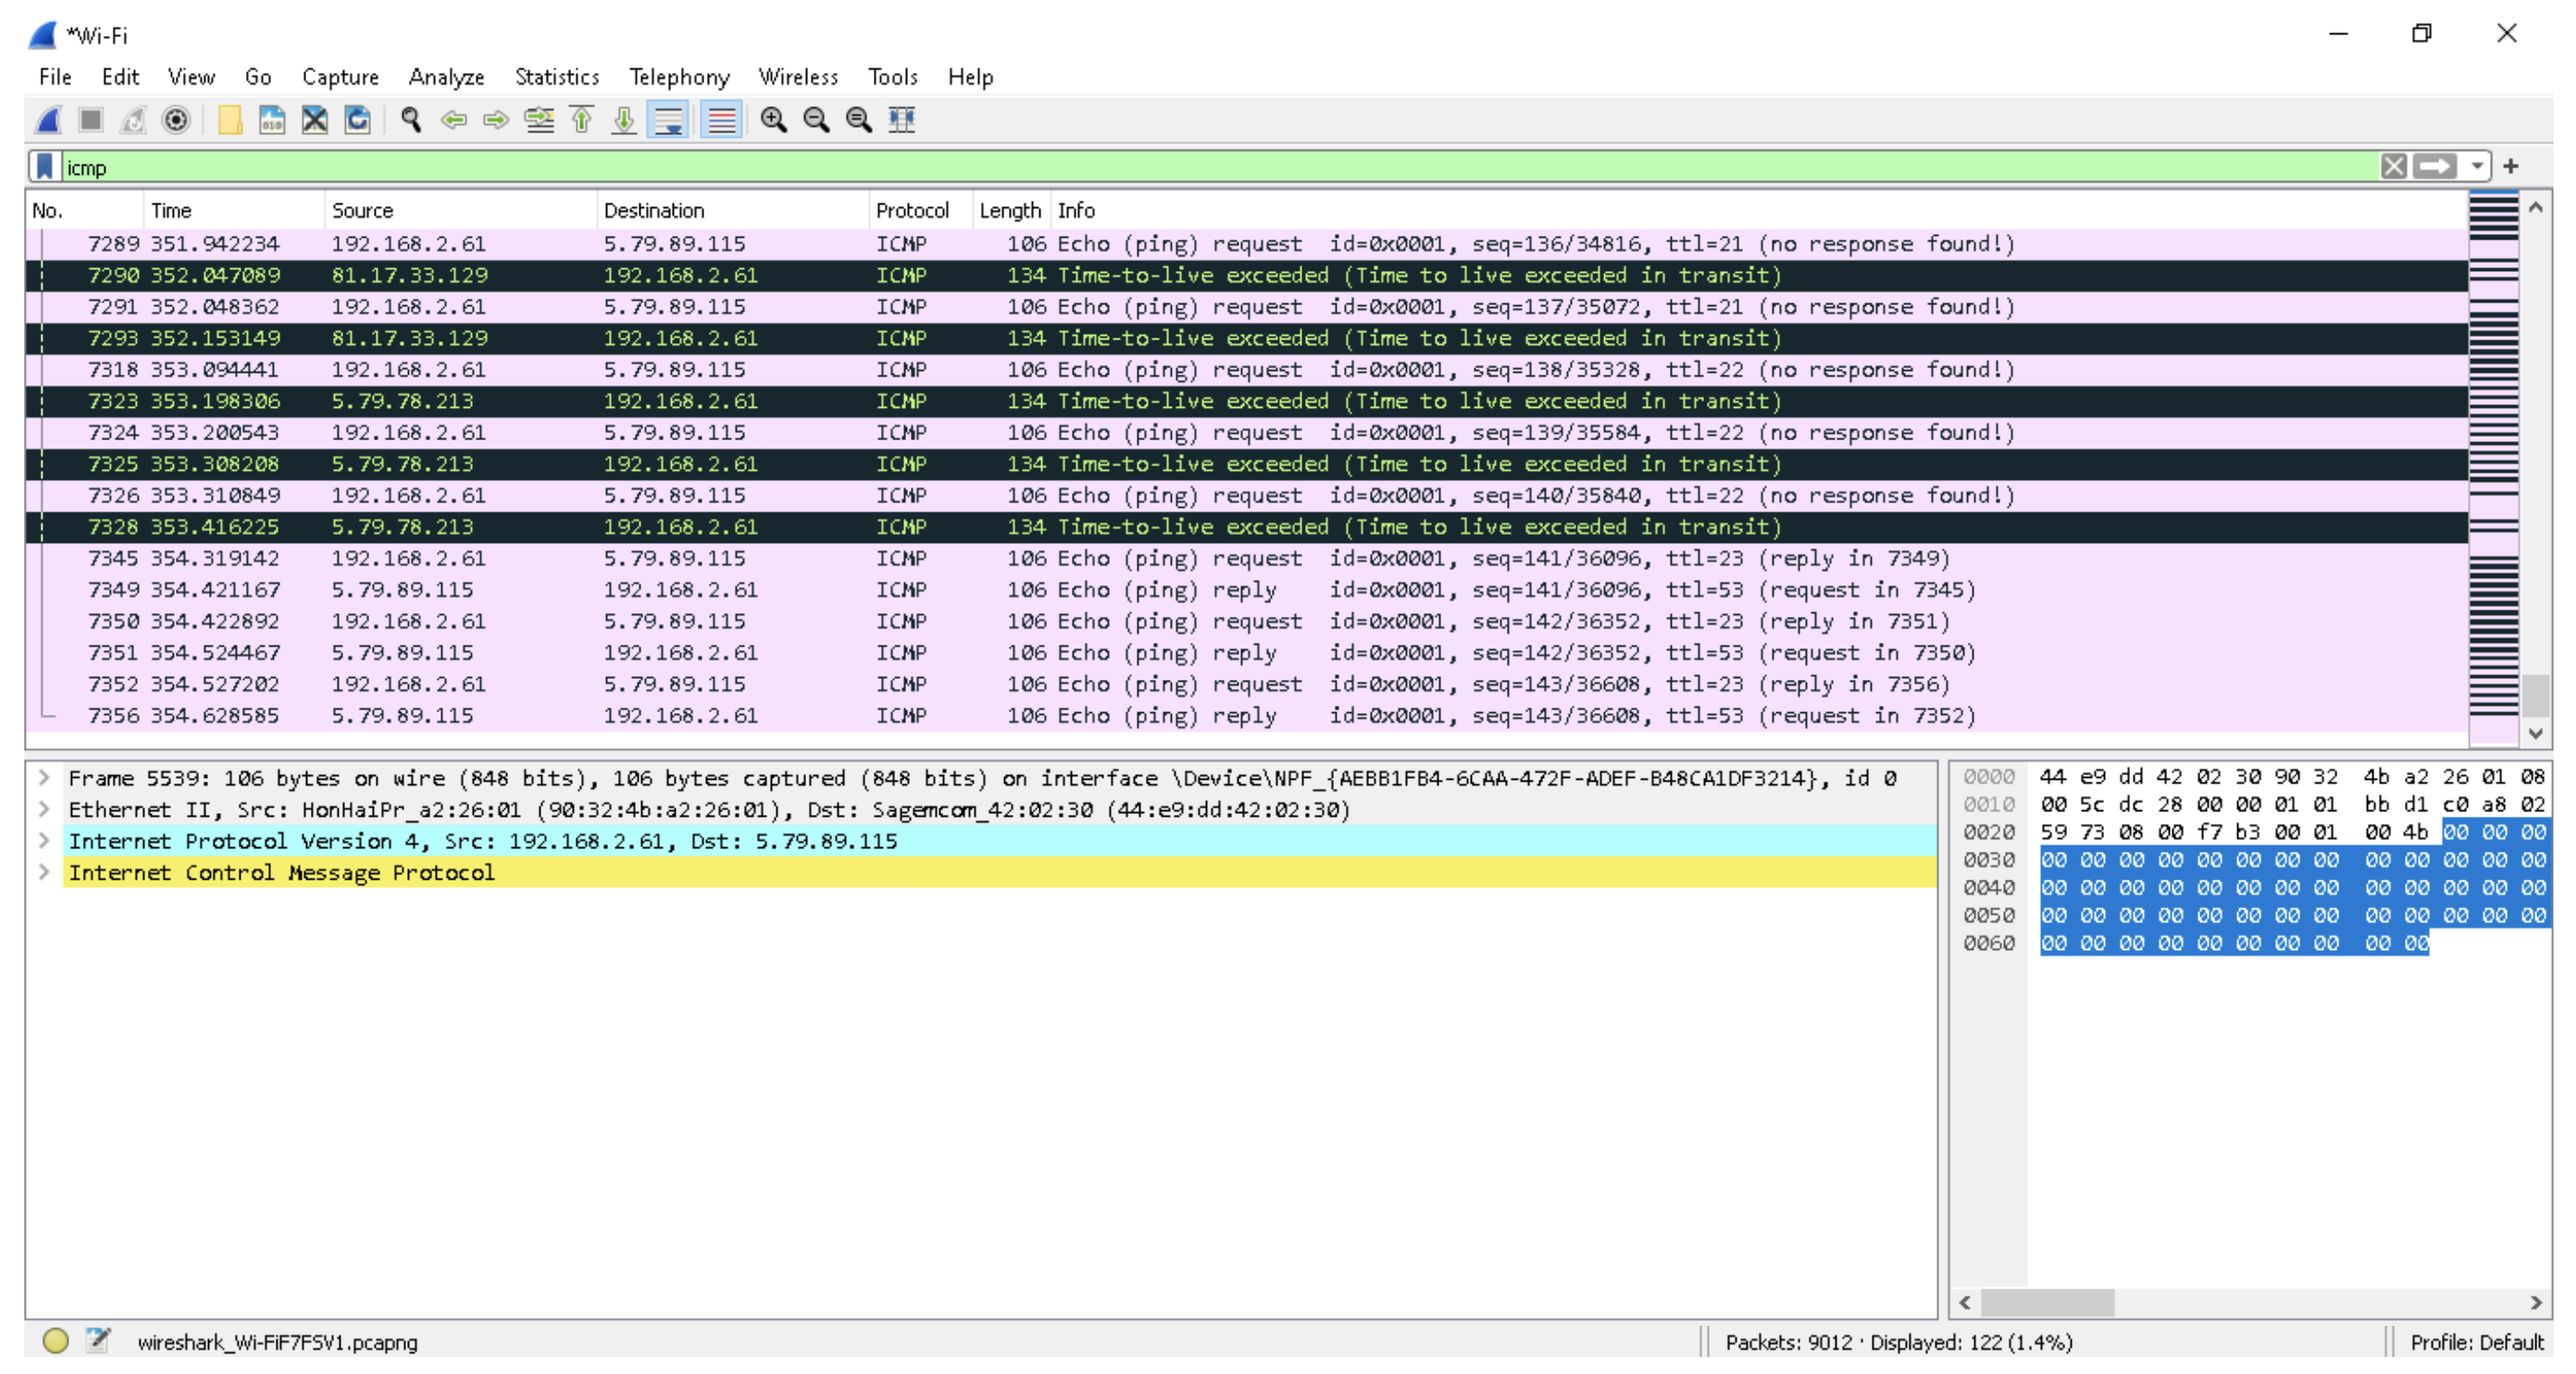
\includegraphics[width=\textwidth]{subfiles/images/PART1_FIG1.png}
    There is a response with 6 ICMP packets in the directory. 66 "echo (ping) request" ICMP packets failed because "no response received" in the last 6 ICMP packets.
\end{proof}
\newpage

\problem{2}
\begin{wts}
    How many probe packets are sent from the source to the destination for each TTL?
\end{wts}
\begin{proof}
    3 research packets for TTL.
\end{proof}
\newpage

\problem{3}
\begin{wts}
    The last few echo-request ICMP packets are followed by the echo-reply ICMP packets. Compare one of them with the corresponding reply. Determine which fields are similar and which fields are different? Explain the reason.
\end{wts}
\begin{proof}
    The first two ICMP packets in the last list have their own public address numbers, the third and fourth, and the fifth and sixth are identical. This is because for every sequence number there is an ICMP Echo Request packet followed by an ICMP Echo Reply packet. We see that it changes "echo (ping) requests" (from source: 192.168.2.61 to destination: 5.79.89.115) and "echo (ping)" responses (from source: 5.79.89.115 up to: 192.168.2.6). ICMP packets.
\end{proof}
\newpage

\problem{4}
\begin{wts}
    What are the TTL values for these last few packets? Determine the number of routers between the source and destination based on these TTL values.
\end{wts}
\begin{proof}
    The TTL values for new packets are 23 for requests and 53 for responses. This means that the packet will go through 23 routers to reach its destination.
\end{proof}
\newpage

\problem{5}
\begin{wts}
    Examine the IP packet header of the last echo-request ICMP packet, what is the value in the “Protocol” field? What does this field indicate?    
\end{wts}
\begin{proof}
    Check the IP header of the last ICMP Echo-Request packet, the value of the "Protocol" field is "ICMP". This field specifies the protocol used in TCP/IP to send errors or responses to communications between IP addresses.
\end{proof}
\newpage

\problem{6}
\begin{wts}
    How many bytes are in this IP header? How many bytes are in the payload of this IP packet? Explain how you determined the number of payload bytes.
\end{wts}
\begin{proof}
    The image printed after this sentence is of utmost importance.\\
    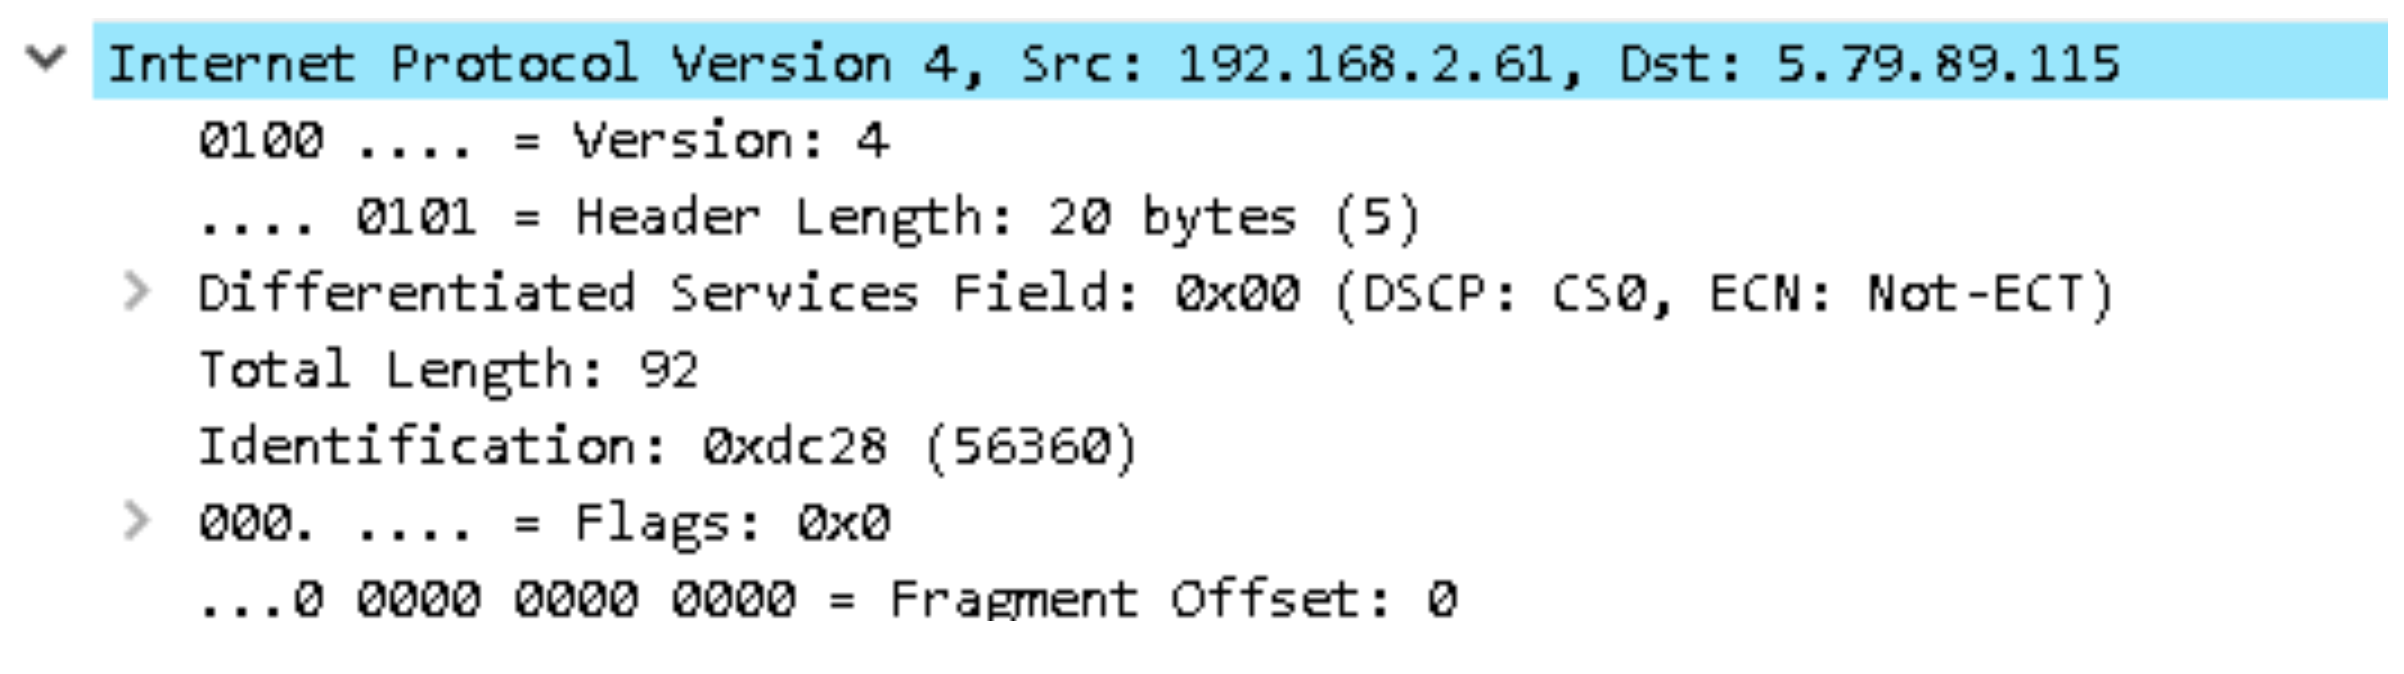
\includegraphics[width=\textwidth]{subfiles/images/PART1_Q6.png}
    From above, it is obvious that the length of the IP header is 20 bytes and the length is 92 bytes, which means the length of user data = length - IP header = 92 bytes - 20 bytes = 72 bytes.
\end{proof}
\newpage

\problem{7}
\begin{wts}
    Has this IP packet been fragmented? Explain how you determined whether or not the packet has been fragmented.
\end{wts}
\begin{proof}
    Consider the following graphic.\\
    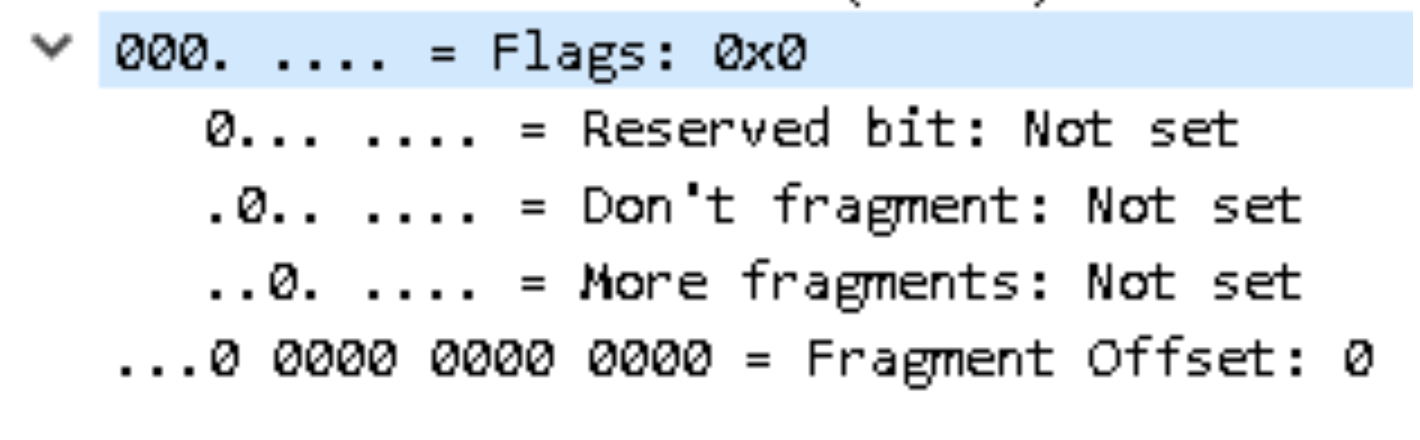
\includegraphics[width=\textwidth]{subfiles/images/PART1_Q7.png}
    Again, the most cursory of surveys of the above image will lead us directly to the conclusion that the IP header is 20 bytes and the length is 92 bytes, ie. A. User data length = Total length - IP header = 92 bytes - 20 bytes = 72 bytes, and it is not fragmented.
\end{proof}
\newpage

\problem{8}
\begin{wts}
    How the IP address of www.acm.org can be found? Determine the packet and the filed in the packet that contains this information.
\end{wts}
\begin{proof}
    The reader should turn their gazes — if for a short moment — towards the two figures below.\\
    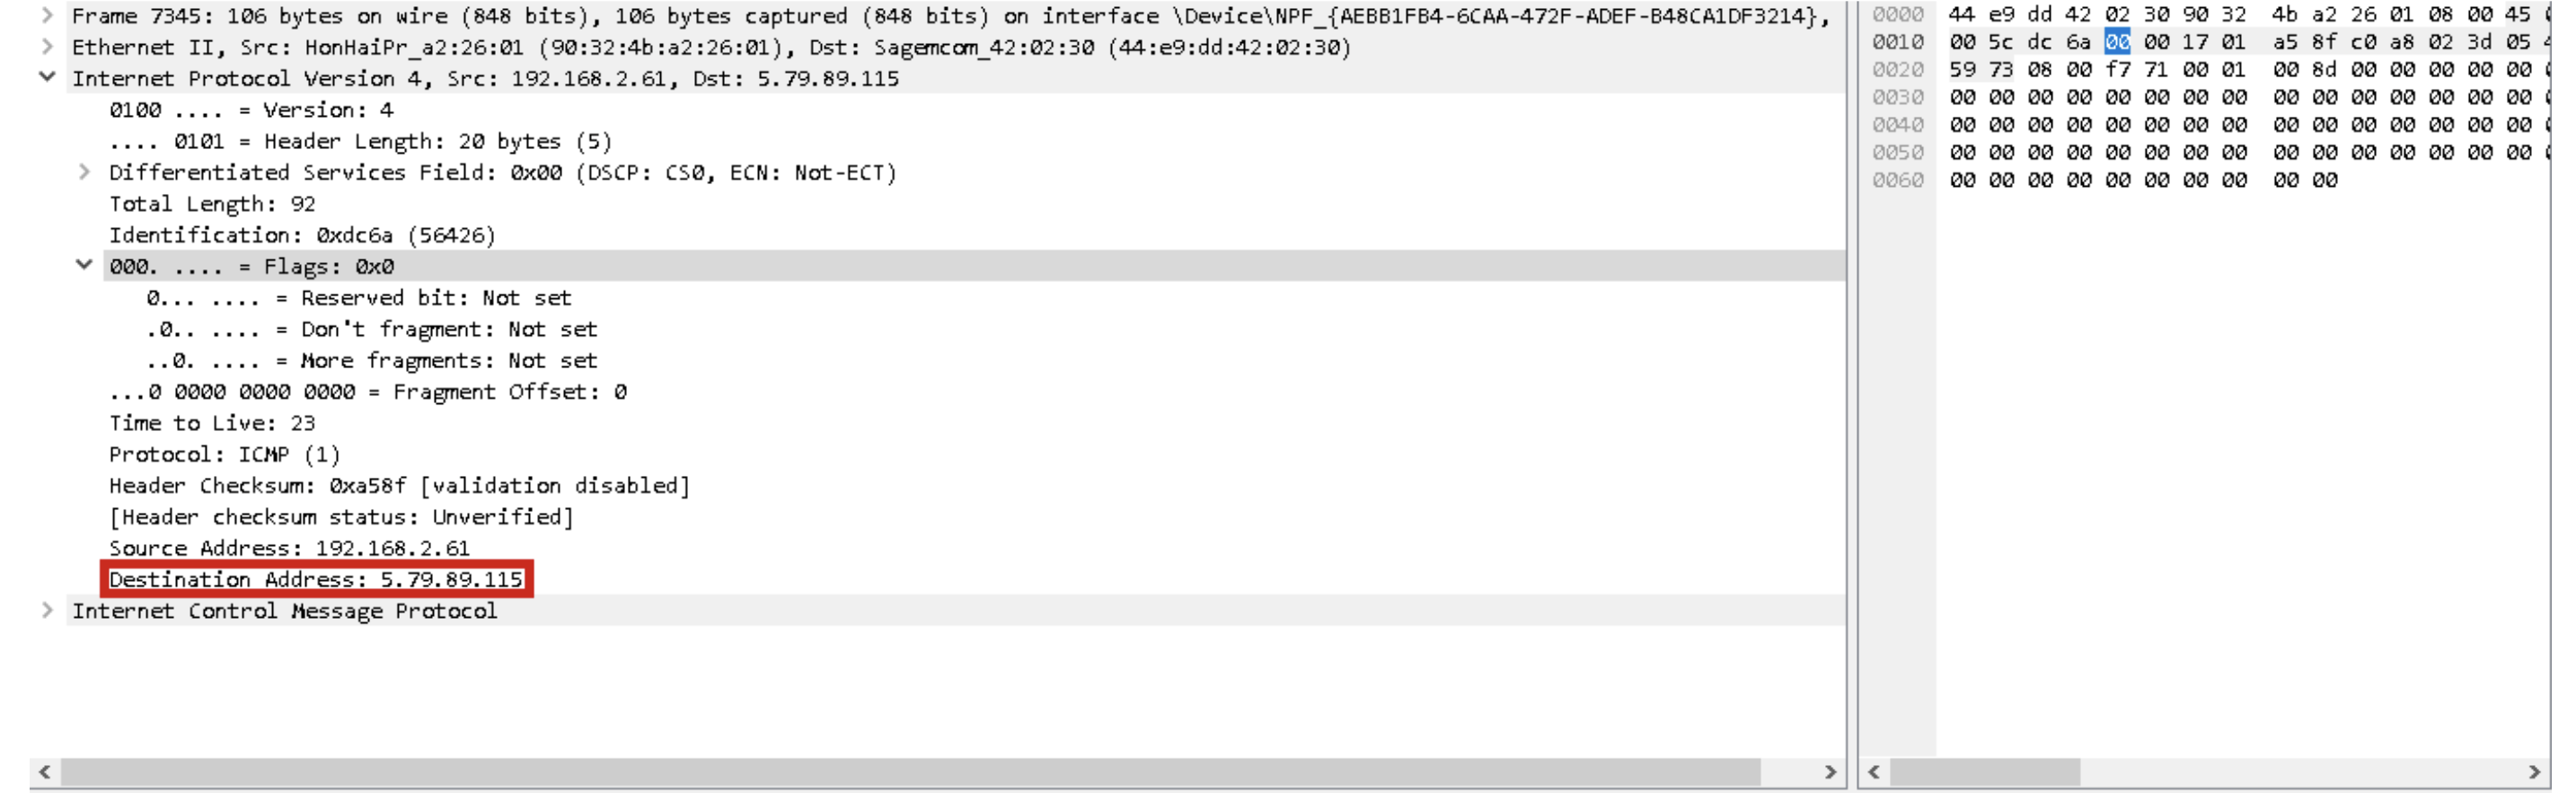
\includegraphics[width=\textwidth]{subfiles/images/PART1_Q8_1.png}
    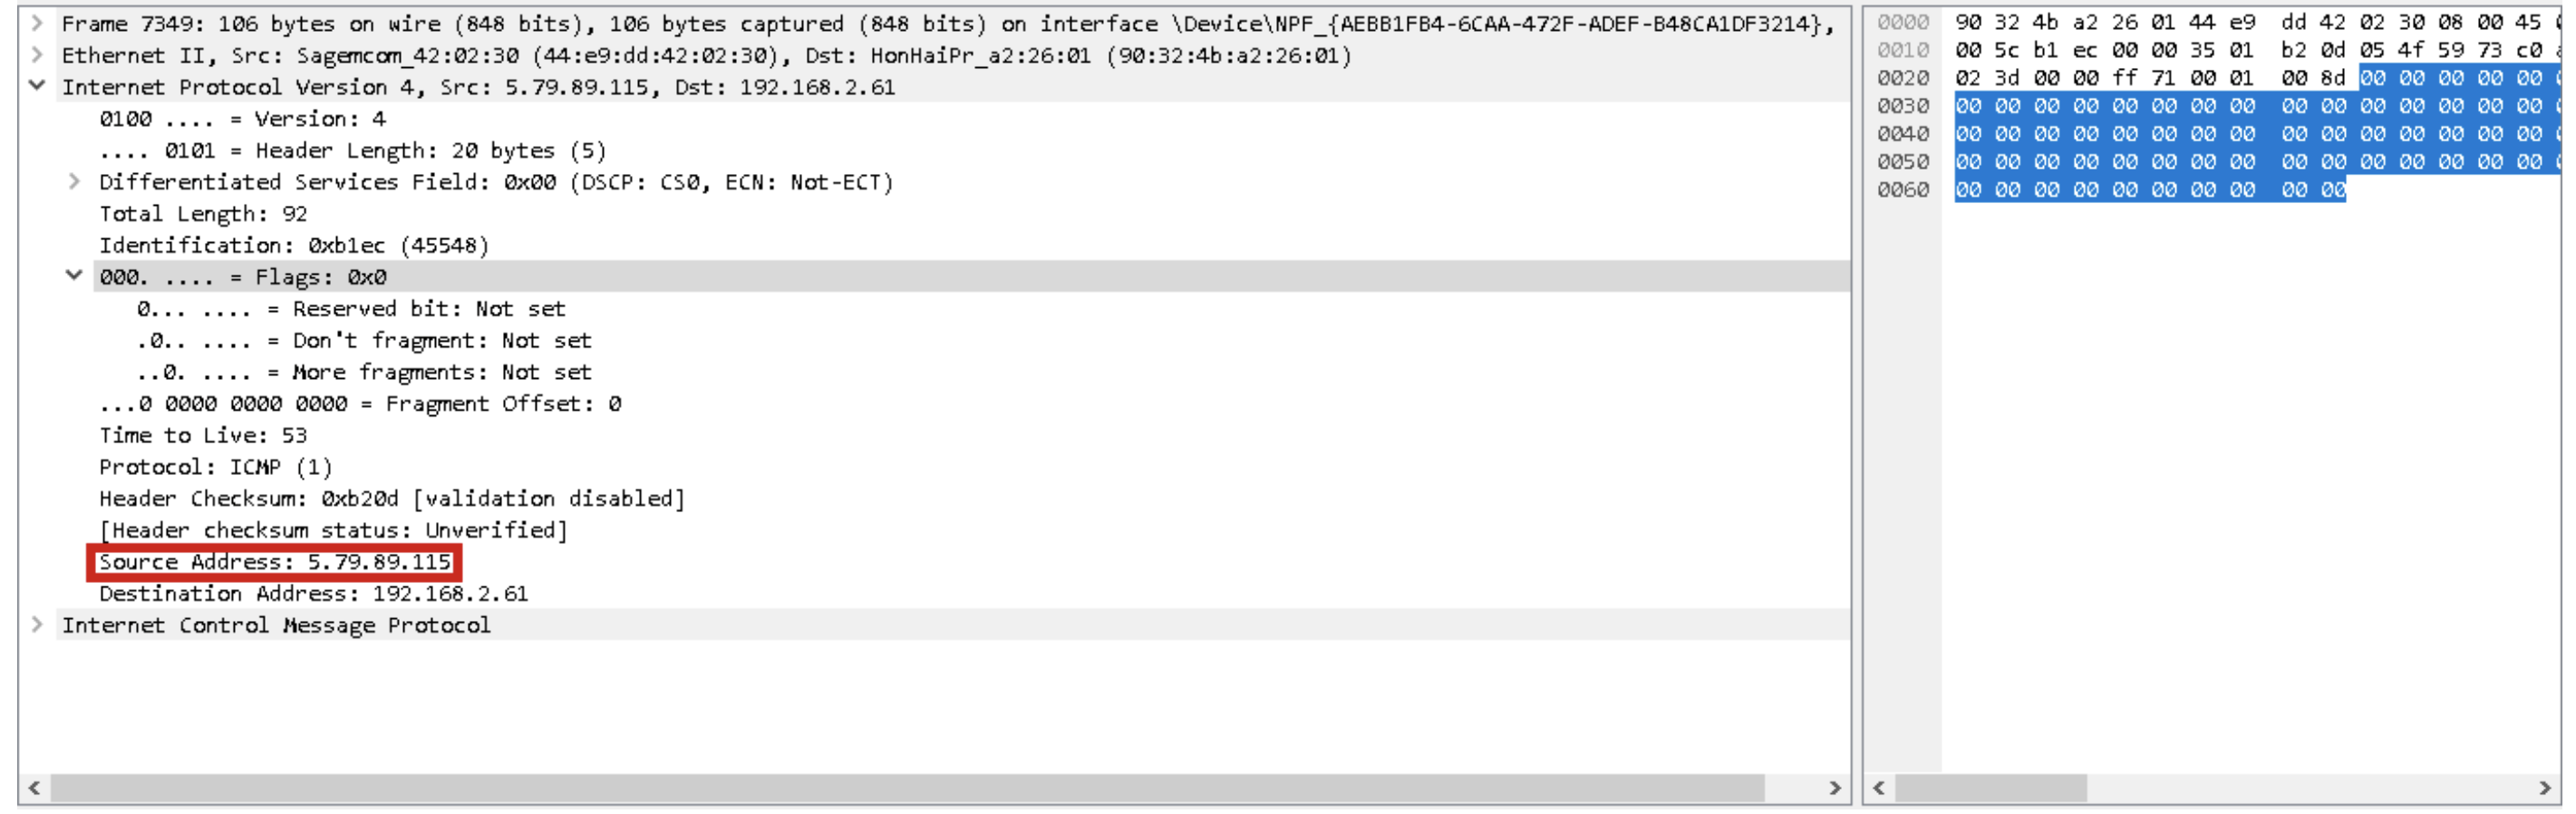
\includegraphics[width=\textwidth]{subfiles/images/PART1_Q8_2.png}
    The IP address www.acm.org can be determined by looking at the destination address of the ICMP Echo Request packet or the source address of the ICMP Echo Reply packet (both ways: 5.79.89.115). This is useful because the target of the echo request and the target of the response sent is the website we are trying to reach (www.acm.org).
\end{proof}
\newpage
\end{document}